\chapter{Applying the PSO to the FAP}
\label{chpt:psoapplicationFAP}
\section{Introduction}
PSO, as discussed previously (see page \pageref{sec:PSO}), is an algorithm that is largely based on the flying behaviour exhibited by a flock of birds. This is why the core of the algorithm is based upon vector mathematics, with new positions and velocities being calculated after each iteration of the algorithm. Thus a D-dimensional vector represents each particle position and is then simulated by flying through the D-dimensional space using the velocity equation (see section~\ref{sec:particleVelocity} on page~\pageref{eq:velocityupdate}).

Most of the problems to which \gls{PSO} has been applied to date have been problems where the position of particles has a constant D-dimensional space. This constant dimensionality introduces an intriguing problem if one wants to apply the \gls{PSO} to an inherent multidimensional problem like the \gls{FAP}. This chapter deals with how the \gls{PSO} was applied to the \gls{FAP}.

First, the particle position representation in the frequency planning domain is defined. This definition of the particle position is important because it plays a central part in the movement of particles through the frequency planning domain. A description is then given of how each position is evaluated as well as the fitness function that the \gls{PSO} will use in the \gls{FAP} domain.

Arguably the most important part of the swarm is how the velocity of a particle is calculated and then moving it to a new position in the problem space. The velocity update is important, as it is the primary means by which the algorithm searches the problem space.

As was discussed in section~\ref{sec:psoonfap}, applying the \gls{PSO} to the \gls{FAP} introduces a variety of challenges. One of the challenges is how exactly one moves a frequency plan towards another frequency plan. This is an important question that needs to be addressed as the \gls{PSO} algorithms have no other way of searching the problem space by any other means.

As mentioned in the previous chapter the FAP is a discrete valued problem and for the \gls{PSO} to operate in the \gls{FAP} space custom operators (called velocity functions in this discussion) had to be developed to enable the particles of the swarm to move. These velocity functions are discussed in section~\ref{sec:velocityFAP}. 

Developing custom velocity functions for the \gls{PSO} was simply not enough to achieve good results with the \gls{PSO}. Therefore more innovations needed to be made to improve the solution quality of the \gls{PSO}. In section~\ref{sec:buildglobalbest} a new mechanism is presented for selecting the global best which enabled the \gls{PSO} to get better fitness values and therefore direct the swarm more towards better solutions. Finally, the chapter will conclude with how the swarm utilises history to produce better results to enable the \gls{PSO} to further improve the solution quality.
\section{Position in the Frequency Planning Domain}
This section presents a description on what a position is in the frequency planning domain. First a frequency plan is defined and the general structure to represent such a plan is provided. The section will conclude with the hard and soft constraints and how the constraints aid in creating a frequency plan that is suitable for a network.

A frequency plan, is almost exactly what the name implies: A plan that outlines frequency usage for a mobile telecommunication network. The benchmark problems that were used to test the developed \gls{PSO} all pertained to cellular phone networks and were presented in section~\ref{sec:FAPBenchmarks}. For cellular networks, the frequency plan outlines which frequency must be allocated to which transceiver. With this basic definition, the problem is deceptive as one naturally assumes that there are an infinite number of frequencies that can be used or the number of frequencies available for assignment is more than the number of transceivers in the network. 

The reality is that there are only a finite number of frequencies available for cellphone transmissions, as was discussed in chapters~\ref{chpt:celltech} and \ref{chpt:fap}. Hence a regulatory body needs to assign wireless spectrum to cellphone network operators for use in their networks. A regulatory body is needed because, if a network operator uses just any frequency it wants, it is bound to interfere with someone else also utilising the same frequency.

A network is not assigned the entire wireless spectrum for wireless communication, but rather only a subset is assigned to the network. If one observes the \gls{FAP} benchmark problems the \gls{PSO} was applied to (see section~\ref{sec:FAPBenchmarks}) for instance Siemens 1, the allotted spectrum is from frequency 16 to 90. Which gives the network operator 74 frequencies to use in its network without considering other constraints. 

Besides the electromagnetic constraints that are also applicable here, there are regulatory constraints, for instance frequencies in the spectrum that are by no means allowed to be used. These frequencies are referred to as globally blocked frequencies and are hard constraints. An in-depth discussion of these constraints was given in section~\ref{sec:Interference}. As discussed in chapters~\ref{chpt:celltech} and \ref{chpt:fap}, a cellphone network is divided into a number of cells, and each cell requires a certain number of transceivers to service its corresponding area. 

The number of transceivers is based on the expected volume of traffic that a particular cell will experience at peak network usage. Some cells might be located in highly populous areas, which means the potential traffic that cell might need to handle during peak network usage is very high and thus the cell has more than one transceiver to handle the potential traffic. With cells that are located in areas that have a low population, the potential traffic the cell might experience during peak network usage is low and thus the cell only has one transceiver to handle potential traffic.

Based on the amount of traffic a cell needs to handle, the number of transceivers differs; thus in a frequency plan not all cells have the same number of transceivers, otherwise a frequency plan can be modelled as a series of constant D-dimensional vectors, where the D represents the number of transceivers. 
\begin{figure}[ht]
	\centering
	\setlength \fboxsep{0pt}
	\setlength \fboxrule{0.5pt}
	\fbox{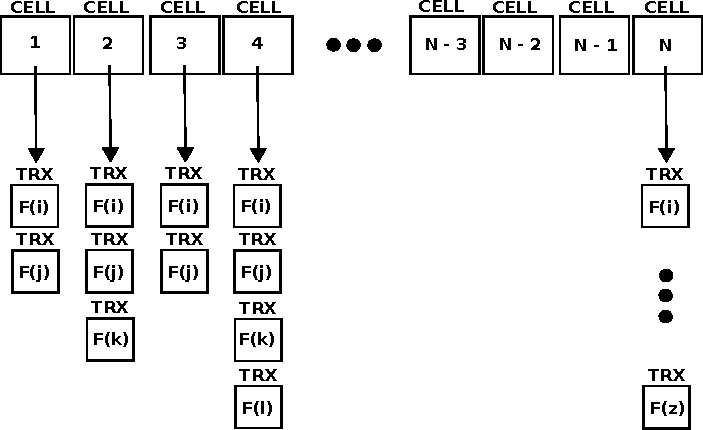
\includegraphics[width=4.8in, height=3.5in]{./pictures/fapPlanDiagram.pdf}}
	\caption{The structure of a frequency plan}
	\label{fig:fapPlan}
\end{figure}
As can be seen in figure \ref{fig:fapPlan} a cellular network can have any number ($N$ in the figure) of cells to attain the desired coverage over the geographical landscape. In the COST 259 benchmark problems the cellular networks have a large number of cells that range from 500 to more than 1000. 

The most important part of the plan is the actual transceivers within each cell. In figure~\ref{fig:fapPlan} it can be clearly seen how the number of transceivers (TRXs) varies from one cell to the next. $F(i)$ is a frequency at position $i$ from the available usable spectrum. 

Based on the structure of the plan depicted in figure \ref{fig:fapPlan} there is no concept of which cell interferes with which other cell and if there is indeed interference; the amount of interference that is experienced. Not all this information is part of the plan. Instead this information, for the purpose of this research is supplied by the COST 259 benchmark. 

The interference information is referred to as the interference matrix. A definition of the structure of an interference matrix was given in section~\ref{sec:Interference}. As discussed, each entry references two cells' entries: Cell A and Cell B. Along with the entry the amount of interference that occurs when Cell B interferes with Cell A is also listed.

A frequency plan is a possible solution to the \gls{FAP}. Therefore in the \gls{PSO} that was developed each particle's position in the solution space is represented by a frequency plan. As illustrated in figure~\ref{fig:fapPlan}, a frequency plan is just a series of cells, where each cell has a set of transceivers; thus in the \gls{PSO} algorithm a plan is actually represented as an array of cells. This enables the algorithm to access particular cells in a plan by index as can be observed in listed algorithms~\ref{alg:velocitymethod1} and ~\ref{alg:velocitymethod2}. 

Before the particles can actually start to move around in the \gls{FAP} space, they first need to be assigned positions. In the developed \gls{PSO} listed in algorithm~\ref{alg:FAPPSO} line 1 the first operation that the algorithm executes is to initialise all the particles in the swarm. A particle position in the algorithm is initialised by assigning it a random position; thus a frequency plan (representing a position) is randomly generated by the algorithm.
\begin{algorithm}[H]
\caption{The \gls{FAP} \gls{PSO} Algorithm}
\label{alg:FAPPSO}
\begin{algorithmic}
\State $s_n$ = Initialize Swarm $s_n$
\While{Termination criterion not met}
	\State EvaluateSwarm($s_n$)
	\State UpdateGlobalBest($s_n$)
	\State UpdateSwarmMovement($s_n$,$gbest$)
\EndWhile
\end{algorithmic}
\end{algorithm}

The position is purely random in that the only considerations made by the position generator are that valid frequencies are assigned to transceivers installed at cells. Thus the generator does not check whether a frequency has already been assigned in the current cell or any other considerations. The intended purpose of the generator is just to place a particle in the problem space, not the premature start of the optimisation process.

Since particles are able to occupy positions in the \gls{FAP} space the \gls{PSO} algorithm is now able to move them around in the problem space. As mentioned previously, moving particles through the frequency plan solution space introduces an interesting problem due to the multidimensionality of a plan. 

A discussion of how particles are moved from one position to another through the solution space is provided in section \ref{sec:velocityFAP}. The next section presents an explanation on the fitness function that determines the desirability of a particular particle's position or rather the frequency plan its position represents.
\section{The Fitness Function}
The fitness function rates the desirability of a particular particle's position in the problem space. As discussed in the previous section, the COST 259 benchmark problems provide an interference matrix that lists the total amount of interference that occurs when a pair of cells interfere. As outlined in the structure definition (see section~\ref{sec:Interference}) each entry in the interference matrix defines a pair of cells that are said to interfere, along with two additional values. 

The first value is referred to as co-channel interference and is the total amount of interference that will occur on the communication link when the allocated frequency of one transceiver, is equal to a transceiver in the other cell that is listed in the interference matrix. The second value is called adjacent channel interference and it is the total amount of interference that will occur on the communication link when the allocated frequency of a transceiver, in one cell, differs by 1 from another frequency allocated to the transceiver from the other cell that is listed in the interference matrix.

Particles move towards other particles because the other particles have indicated (through information sharing) that the positions they occupy are very lucrative and thus they have found potentially good solutions. The particles in the developed \gls{PSO} share information based on the star social network structure. The only way particles can know the lucrativeness of the position they occupy is if the position is evaluated with a fitness function. Thus the lucrativeness of a position is actually the fitness value obtained from the fitness function.

Since a particle position is defined as a frequency plan, a procedure is needed that calculates the fitness of a frequency plan. With the \gls{FS-FAP} the primary concern is to keep interference to a minimum. Therefore in the \gls{PSO} that was developed the fitness value is the total amount of interference generated by all the cells with their allocated frequencies. 

The evaluation procedure goes through each pair of cells defined in the interference matrix where it looks up both cells in the frequency plan. The second cell is said to interfere with the first cell. Therefore each transceiver in the first cell is checked against all the transceivers of the other cell. Depending on whether the frequencies differ from each other, the fitness procedure adds either co-channel or the adjacent channel interference to a summing variable. This procedure is mathematically defined in chapter 3 (see page \pageref{E:costFunction} for the formal equation) and algorithm~\ref{alg:fapcost} is the pseudo code of the implemented equation used by the \gls{PSO} . 

\begin{algorithm}
\caption{FAP Cost Function}
\label{alg:fapcost}
	\begin{algorithmic}[1]
	\Require normalCell
	\Require interferingCell
	\State $totalInterference \leftarrow $0
	\For{Each TRX $trx_i$ in interferingCell}
		\For{Each TRX $trx_j$ in normalCell}
			\State $interference \leftarrow 0$
			\State $difference \leftarrow$ $|trx_i - trx_j|$
			\If{difference is 0}
            \If{\emph{coChannelInterference} $\leq$ \emph{minInterferenceThershold}}
					\State $interference \leftarrow interference + 0$
				\Else
                \State \emph{interference} $\leftarrow$ \emph{interference} + \emph{coChannelInterference}
				\EndIf
			\Else
            \If{difference is 1}
                \If{\emph{adjChannelInterference} $\leq$ \emph{minInterferenceThershold}}
                    \State \emph{interference} $\leftarrow$ \emph{interference} + 0
					\Else
                    \State \emph{interference} $\leftarrow$ \emph{interference} + \emph{adjChannelInterference}
					\EndIf
				\EndIf
			\EndIf
            \State \emph{totalInterference} $\leftarrow$ \emph{totalInterference} + \emph{interference}
		\EndFor
	\EndFor
	\end{algorithmic}
\end{algorithm}

As can be seen in algorithm~\ref{alg:fapcost} not all interference values are added to the total amount of interference variable. The COST 259 benchmarks define a minimum tolerable interference variable. This means that if a given interference value is either equal to or less than this defined value the interference generated is negligible and can be disregarded as it will not have a noticeable impact on the communication link. The following section discusses how particles are moved from one iteration to the next using frequency plans as positions in the solution space.
\section{Velocity Function for Frequency Planning}
\label{sec:velocityFAP}
The velocity function is arguably the core of the \gls{PSO} algorithm. It is the procedure by which particles in the swarm move from one point to another in the solution space. 

The velocity function does not blindly move a particle from one point to another, but instead it takes the particle history into account as well as the best particle in the swarm. Therefore the velocity function is the core means by which the swarm explores the solution space. A more thorough explanation is provided in section~\ref{sec:particleVelocity}.

The development of a velocity function that is suitable for particles to move from one frequency plan to another is covered next. The section will start off with the first velocity function that was developed. With each method discussed, the problems associated with it will also be mentioned. This section will conclude with the second method that was developed and that is also the primary method the developed \gls{PSO} uses.

\subsection{Movement in the Frequency Planning Domain}
The standard velocity equation works on the basis of vector mathematics. Each particle has a velocity and position, which is represented by a standard mathematical vector. The standard equation alters the direction of the particle to move to a more promising position in the solution space that is in the general direction of the global best particle and a previous personal best position the particle held.

Vector mathematics has standard basic operations defined for adding, subtracting and multiplying; hence applying the \gls{PSO} to problems that are either mathematical functions or problems that map well to the vector domain is a defined process. With regard to the frequency planning domain an important question needs to be answered: How can one multidimension frequency plan be moved to another?

With any difficult problem it is better to break the problem down into its most basic constructs and then solve each piece individually until the problem as a collective is solved. This technique is also commonly known as divide and conquer. This technique was first applied to the nature of a frequency plan.

A frequency plan is a plan that consists of a series of different cells that are in use in the network. The plan specifies the frequencies that each individual transceiver installed at a cell must use for communication. Thus a frequency plan can be broken up into three important constructs:
\begin{enumerate}
\item A plan is a list of different cells.
\item Each cell in a plan has a list of transceivers that it has installed.
\item Each installed transceiver has a single number allocated to it called the frequency. This frequency is used for communication.
\end{enumerate}

As discussed previously, a position is a frequency plan and each particle has a current position and a best position. A visual depiction of a particle position is presented in figure~\ref{fig:fapparticlepos}. The global best particle is also depicted in the figure. In the figure, position 1 represents a particle. The current compartment in the particle represents the current position and hence a frequency plan. The best compartment represents the best position found and hence the best frequency plan found thus far by the particle. When providing examples on how any of the following velocity methods operate, figure~\ref{fig:fapparticlepos} is used as reference point.
\begin{figure}[ht]
	\centering
	\setlength \fboxsep{0pt}
	\setlength \fboxrule{0.5pt}
	\fbox{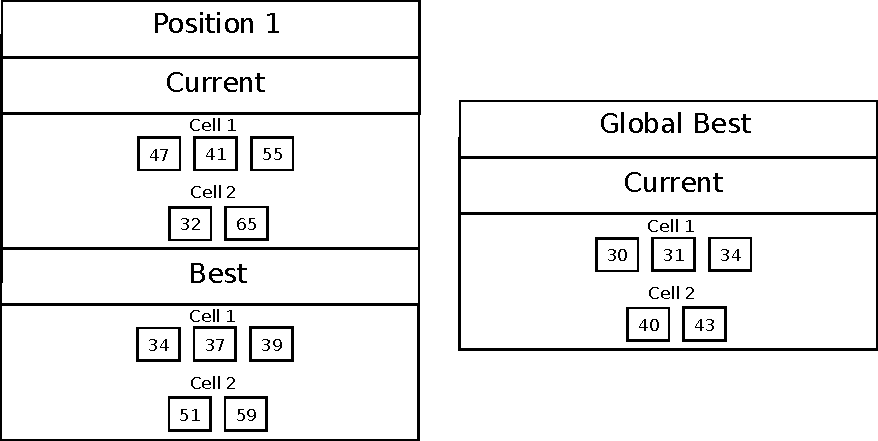
\includegraphics[width=4.8in, height=3.00in]{./pictures/FAP_Particle_Positions.pdf}}
	\caption{FAP PSO Particle Position and Global Best Position}
	\label{fig:fapparticlepos}
\end{figure}

Now that a frequency plan has been broken up into its constructs, the question of how to move one frequency plan to another can be rephrased. How does one move a frequency allocated to a \emph{transceiver} in a particular \emph{cell} of one frequency plan to another frequency of the \emph{same} transceiver and cell in another \emph{different} plan? An important realisation needs to be noted here. In the \gls{PSO} at any one time the algorithm is only considering two positions and for the \gls{FAP} the two positions are frequency plans. Both plans are \emph{identical} except for the specific frequencies that transceivers use. Thus a cell that exists in the one plan, also exists in another plan. Both the cells have exactly the same number of transceivers installed; only the frequencies of each individual transceiver uses for communication differ.

Using this realisation, the conclusion can be made that the velocity equation can only work with the frequencies assigned to transceivers. Therefore a potential velocity equation mechanism needs to operate on the finest granularity of a frequency plan, i.e. the frequencies.

The principle on which the first velocity method developed is based, is for the movement of the swarm to be at a much finer granularity and hence movement is based on frequencies. Therefore when a particle needs to move towards a global best particle, the velocity procedure goes into the intricate details of the particle wanting to move and the global best particle. The procedure goes into each cell defined in the frequency plan represented by the standard particle as well as the global best particle to be able to access each installed transceiver.

To be able to move from one frequency plan to another by utilising the standard velocity equation, the equation needs to be broken up into its smaller operations. In this way, small operations can be developed that perform the same function as the individual parts. The velocity equation in section~\ref{sec:particleVelocity} can be broken up into the following parts:
\label{lst:velocitybreakup}
\begin{itemize}
\item \textbf{Subtraction} \\SubtractionResultPbest: $pbest - x_i(t)$\\SubtractionResultGbest: $gbest - x_i(t)$
\\
\item \textbf{Multiplication} \\MultiPbestResult: $c_1\phi_1 * SubtractionResultPbest$\\MultiGBestResult: $c_2\phi_2 * SubtractionResultGbest$ 
\item \textbf{Addition}\\$v_i(t) + MultiPbestResult + MultiGBestResult$
\end{itemize}
There are no mathematical constructs that define how two frequency plans are added together or subtracted, let alone multiplied. As discussed earlier, a frequency plan is just a series of cells that have frequencies. These frequencies are numbers that internally are just integers and there are mathematical constructs that define how two integers should be added, subtracted or multiplied. Both velocity methods that were developed utilise the basic principle that on a fine granularity of a frequency plan one is merely working with integers.


The first velocity method is listed in algorithm~\ref{alg:velocitymethod1}. Velocity method 1 works on the principle of moving one cell in a particular frequency plan to the same cell in a different frequency plan. As noted earlier, the cells are the \emph{same}, but the frequencies that have been allocated to each transceiver within a cell differ. Thus in velocity method 1, each cell has an array of transceivers. The array of transceivers contains the individual frequency numbers that have been allocated to a cell.

Before the algorithm is presented, the operations used for addition, subtraction, multiplication and multiplication with a scalar needs to be defined. The following equations formulate all of these operations and are used by Velocity method 1.
\begin{align}
    \Delta c_{ij} &= f(c^1_{ij}) + f(c^2_{ij})\label{eq:arrayAdd}\\
    \Delta c_{ij} &= f(c^1_{ij}) - f(c^2_{ij})\label{eq:arraySubtract}\\
	\Delta c_{ij} &= f(c^1_{ij}) * f(c^2_{ij})\label{eq:arrayMultiply}\\
    \Delta c_{ij} &= f(c_{ij}) * s \label{eq:arrayScalar}\\
    \text{where, }c &\in \{c_{00},c_{01},c_{10}, \dots, c_{ij}\} , \forall i,j,s \in \mathbb{N}, i \leq \text{MaxCells}, j \leq t(c_i)\nonumber\\ 
    p_i &\in \{\{c_{01},c_{02},\dots,c_{ij}\}_1,\{c_{01},c_{02},\dots,c_{ij}\}_2, \dots,\{c_{01},c_{02},\dots,c_{ij}\}_k\}\nonumber
\end{align}
In the above equations $c^1$ and $c^2$ represent different frequencies plan positions. The function $f$ retrieves the frequency assigned to a TRX $c_{ij}$. MaxCells is the maximum amount of cells in the frequency plan. The function $t$ retrieves the total amount of TRXs installed at a particular cell $c_i$. The variable $s$ in equation~\ref{eq:arrayScalar} is any scalar value. The variable $p_i$ represents a particle in the swarm and $k$ is the max swarm size. Now that all the equations have been defined, the algorithm can be represented. 

Velocity method 1 is depicted in algorithm~\ref{alg:velocitymethod1}. The algorithm moves one array of transceivers to another array of transceivers. The variable $r$ in algorithm~\ref{alg:velocitymethod1} below is a random scalar value. In each of the equations the particular arithmetic operation is applied to the same TRX found in both frequency plans. The first method that is used to calculate the velocity of a frequency plan, is the first basic operation defined in the velocity equation, namely subtraction, and utilises equation~\ref{eq:arraySubtract}.
\begin{algorithm}[H]
\caption{Velocity Method 1}
\label{alg:velocitymethod1}
	\begin{algorithmic}[1]
        \Require currentParticle -- The particle that needs to move (\emph{fromPosition})
        \Require globalBestParticle -- The particle to move towards (\emph{toPosition})
	\State $pbest \leftarrow $Particle best position
	\State $gbest \leftarrow $globalBestParticle position
	\State $pBestSubtractResult \leftarrow currentParticle - pbest$ with equation~\ref{eq:arraySubtract}
	\State $gBestSubtractResult \leftarrow currentParticle - gbest$  with equation~\ref{eq:arraySubtract}
    \State $a \leftarrow localCoeff \times pBestSubtractResult \times r$ using equation~\ref{eq:arrayMultiply} and~\ref{eq:arrayScalar}
    \State $b \leftarrow globalCoeff \times gBestSubtractResult \times r$  using equation~\ref{eq:arrayMultiply} and~\ref{eq:arrayScalar}
	\If{first time velocity is calculated for current Particle}
		\State $v \leftarrow a + b$ using equation~\ref{eq:arrayAdd}
	\Else
		\State $abAdditionResult \leftarrow a + b$ using equation~\ref{eq:arrayScalar}
		\State $v' \leftarrow abAdditionResult + v$ using equation~\ref{eq:arrayAdd}
		\State $v \leftarrow w \times v'$ using equation~\ref{eq:arrayScalar}
	\EndIf
	\State $currentParticle \leftarrow v + currentParticle$ using equation~\ref{eq:arrayAdd}
	\State SanatizePosition(currentParticle)
	\end{algorithmic}
\end{algorithm}

To better understand how velocity method 1 operates an example will now be presented using figure~\ref{fig:fapparticlepos} as the example position and example global best. Note that in following example, only $cell_1$ is considered for the current, personal and global best position.
\begin{align}
    pbest_1 &= \{34,37,39\} \nonumber \\
    gbest_1 &= \{30,31,34\} \nonumber \\
    cell_1 &= \{47,41,55\} \nonumber \\
    pbestSubtractResult_{11} &= cell_{11} - pbest_{11} \nonumber \\
                        &= 47 - 34 \nonumber \\
    gbestSubtractResult_{11} &= cell_{11} - pbest_{11} \nonumber \\
                        &= 47 - 30 \nonumber \\
    pbestSubtractResult_{12} &= cell_{12} - pbest_{12} \nonumber \\
                        &= 41 - 37 \nonumber \\
    gbestSubtractResult_{12} &= cell_{12} - pbest_{12} \nonumber \\
                        &= 41 - 31 \nonumber \\
    pbestSubtractResult_{13} &= cell_{13} - pbest_{13} \nonumber \\
                        &= 55 - 39 \nonumber \\
    gbestSubtractResult_{13} &= cell_{13} - pbest_{13} \nonumber \\
                        &= 55 - 34 \nonumber \\
    r &= 0.725 \nonumber \\
    pbestSubstractResult &= \{13,4,16\} \nonumber \\
    a &= 0.5 \times pbestSubtractresult \times r \nonumber \\
    &= \{4, 1, 5\} \nonumber \\
    gbestSubtractResult &= \{17,10,21\} \nonumber \\
    r &= 0.654 \nonumber \\
    b &= 0.4 \times gBestSubtractResult \times r \nonumber \\
    &= \{4,2,5\} \nonumber \\
    abAdditionResult &= \{4,1,5\} + \{4,2,5\}  \nonumber \\
                    &= \{8,3,10\} \nonumber \\
    newVelocity &= abAdditionResult \times 0.5 \nonumber \\
                &= \{4,1,5\} \nonumber \displaybreak[4] \\
    cell_1 &= cell_1 + newVelocity \nonumber \\
    &= \{47,41,55\} + \{4,1,5\} \nonumber \\
    &= \{51, 42, 60\} \nonumber \\
\end{align}

In the following discussion the \emph{fromPosition} is the position of the currentParticle. The \emph{toPosition} is the position the currentParticle must move towards. The toPosition in this discussion is the position of the \emph{globalBestParticle}.
The algorithm operates on every cell in the frequency plan. The algorithm starts off by selecting the first cell in the fromPosition and the same for the toPosition. 

Once the cell has been selected the algorithm obtains the exact same transceiver in the toPosition frequency plan. This operation is quick, as the two plans are identical except for the frequencies assigned to transceivers for each cell. Thus the algorithm is able to refer to the cell and specific transceiver in the toPosition plan by the same index it utilises to access the cell and transceiver in the fromPosition. After all the cells in the frequency plan has been processed the algorithm proceeds to the next phase.

After the subtraction, a position is returned which is the result of subtracting the fromPosition from the toPosition. Subtraction of two frequency plan positions occurs on lines 4 -- 5. Using the subtraction result the velocity method 1 algorithm is now ready to apply the next operation in the velocity update equation, namely multiplication by using equations~\ref{eq:arrayMultiply} and \ref{eq:arrayScalar} which are applied in lines 5 -- 6.

In the multiplication stage of the velocity update operation, the local and global coefficients defined for the \gls{PSO} are multiplied into a position, i.e. frequency plan. The coefficient are scalar values and therefore a different method needs to be used to multiply a scalar value with a frequency plan. Equation~\ref{eq:arrayScalar} is used to multiply scalar values with frequency plans. Multiplying a frequency plan results in another frequency plan. Scalar values need to be multiplied in the following cases in the velocity update.
\begin{itemize}
\item The inertia case: $w \times v(t+1)$, where $w$ is the inertia value and $v(t+1)$ is velocity that has already been calculated for a particular particle $t$. Note, a velocity that has been calculated is still a frequency plan. In the algorithm, inertia is applied in line 12.
\item Standard velocity calculation randomisation case: As can be observed from the velocity equation~\ref{eq:velocityupdate} and also from the multiplication bullet point on page~\pageref{lst:velocitybreakup}, the equation requires that a position be multiplied by a coefficient $c_1$ or $c_2$ and then a random value $\phi_1$ or $\phi_2$. 
\end{itemize}

Regardless of which case is executed, the actual operation that is performed is integer multiplication, which therefore means that even though the inertia and random numbers are decimal, the fractional component of the result is discarded. Frequencies are integers so the loss of the fractional component is warranted as it is of no use. Note that it is highly probable that the frequencies depicted in the plan are out of the defined spectrum boundary. As per the last bullet point on page~\pageref{lst:velocitybreakup} the last basic operation that occurs in the velocity equation is the addition of frequency plans. Note that the calculated velocity is still considered to be a frequency plan on its own.

The addition operation is the last operation that occurs in the velocity equation and is also the only operation that occurs when the resultant velocity is applied to the current position of a particle as in equation~\ref{eq:positionupdate}. The addition is performed by the algorithm in line 14. Since the addition operation is also used in the final position update of the particle, it is last opportunity where frequencies can be bounded.  The purpose of the bound operation is to keep the frequencies within valid value ranges. In equation~\ref{eq:arrayAdd} the frequencies are bounded using function $b$ defined in equation~\ref{eq:boundEq} which is formulated in the following section.
\subsection{Keeping Frequencies Bounded}
The previous section discussed the first velocity method that was developed. The velocity method is important as it calculates the direction and next position of a particle in the problem space, where the problem space is the \gls{FAP} and a position of a particle is a possible frequency plan. With the velocity method defined, the swarm is now able to move around in the problem space, but this alone is not enough. The swarm has no concept of the constraints that are imposed inherently by the domain as well as the network for which a frequency plan is being created.

Due to the swarm not having a concept of the constraints a constraint handling mechanism needs to be used. Each of the methods discussed in this section fall under the category of using the \emph{repair method} which is discussed in section~\ref{sec:chm}. The first method that was developed was the BoundValue method and is formulated in equation~\ref{eq:boundEq}.

\begin{align}
\label{eq:boundEq}
    \Delta b(c_{ij}) &= 
    \begin{cases}
    F_{min} + f(c_{ij}) \bmod F_{max} &, \text{if $f(c_{ij}) \geq F_{max}$}\\ 
    b(f(c_{ij}) + F_{min}) &, \text{if $f(c_{ij}) \leq F_{min}$}\\ 
    \end{cases}
\end{align}
Where $F_{min}$ and $F_{max}$ are the minimum and maximum frequencies of the defined spectrum. The function $b$ is the BoundValue function. The constraints that are imposed are part of the spectrum that may under no circumstances be used anywhere in the network, which as discussed in chapter~\ref{chpt:fap} is known as globally blocked frequencies. Some frequencies that are only allowed to be used in certain parts of the network are known as locally blocked frequencies. Then of course the swarm also needs to take into account the electromagnetic constraints.

The velocity function used by the \gls{PSO} needs to be altered to make the swarm more aware of the domain it is operating in and hence keep the particle positions bounded within the allowable search space. By not bounding particle positions in the \gls{FAP} problem space, transceivers of some cells might be assigned a frequency that is not allowed or not even allocated to the network. The \gls{PSO} will accept this assignment since the fitness function operates on the assumption that under no circumstances will these invalid frequencies be assigned and thus does not penalise invalid assignments.

To keep assigned frequency values to transceivers in the allocated spectrum of the network a boundary check needs to be added to the velocity method. The purpose of the boundary check is to validate all assignments in a position, i.e. the frequency plan that a particle currently occupies, and if any assignments violate the defined boundary constraints then it must take the violating value and modify it to be in the acceptable value range.

The boundary check that is used by velocity method 1 operates on the basis that for any range of values there is a defined lower bound (a minimum value) and upper bound (a maximum value). The frequency boundary check is only applied when one of the following conditions are met after the calculated velocity has been applied to the current position:
\begin{itemize}
\item If a frequency allocated to a transceiver is above the maximum allowable frequency (upper bound) given to the network. 
\item If a frequency allocated to a transceiver is below the minimum allowable frequency (lower bound) given to the network.
\end{itemize}

As can be seen from equation~\ref{eq:boundEq}, a mod operation is applied to the value to bring it within the allowable range. The integer mod operation is similar to integer division, the only difference being in the result that is produced. Division produces the result of two numbers being divided. Mod produces the remainder of two numbers being divided. If two numbers divide perfectly into one another there will not be any remainder; if the numbers do not divide perfectly into one another there will be a remainder. 
\begin{align}
	10 \bmod 50 =& 10 \nonumber \\
	60 \bmod 50 =& 10 \nonumber \\
	50 \bmod 50 =& 0 \nonumber \\
	100 \bmod 50 =& 0 \nonumber \\
	35 \bmod 50 =& 35 \nonumber 
\end{align}

As can be seen in the above example mod operations, any value that is modded will be kept in the range $[0,50]$. With regard to frequencies, the following occurs: If, for instance, the maximum allowable frequency is 50, and the transceiver has a frequency value (after velocity) of 56, the 56 value is modded by 50 to produce a value of 6. This modded value is then added to the minimum allowable frequency. In essence, the value is wrapped around to always be within acceptable range. 

The difficult case is when the frequency value is lower than the minimum frequency given to the network. This is because modding the frequency value has no effect. For example, if the lowest allowable frequency is 20 and the transceiver value after movement is 15, modding the transceiver value of 15 by 20 has no effect. To solve this, the following options are then considered:

\begin{enumerate}
\item First subtract the lower value from the minimum allowable frequency. Then add the result to the minimum allowable frequency. The resultant value is checked again as to whether it oversteps the bounds of the maximum allowable frequency and is bounded accordingly.
\item Add the lower value to the minimum allowable frequency. The resultant value is checked as to whether it oversteps the bounds of the maximum allowable frequency and is bounded accordingly.
\item Repeatedly subtract the lower value from the maximum allowable frequency until the resultant frequency is within the acceptable frequency range.
\end{enumerate}

An important notion to consider is that, based on the velocity equation, it is entirely within the realm of possibility that a frequency value after movement might contain a negative value. As can be seen in the second case of equation~\ref{eq:boundEq}, if the assigned frequency is less than $F_{min}$ then $F_{min}$ is added to the frequency and the boundary function is applied again. Therefore, the boundary function is repeatedly called until the frequency to be bounded comes into a valid range.

Using this bound method to keep frequencies within the acceptable range of frequencies add unnecessary complexity. This complexity can be completely avoided by using frequency index values rather than actual frequency values for frequency plans. How indices are used instead of raw frequency values is discussed in the following section.
\subsection{Using Indices instead of Frequencies}
\label{sec:velocityFAP2}
As discussed in section~\ref{sec:velocityFAP} and as can be observed from algorithm~\ref{alg:velocitymethod1}, the first velocity method that was developed for the \gls{PSO} worked with raw frequency values. This is not ideal since upon closer inspection the frequency range that the swarm used to move around was indeed incorrect. The bound value function only keeps frequencies within a minimum and maximum allowable frequency range, but globally blocked frequencies and locally blocked frequencies can be in between this minimum and maximum frequency range. 

With velocity method 1 i.e algorithm~\ref{alg:velocitymethod1} and the \gls{PSO} using raw frequency values, the swarm increasingly moved towards allocating these blocked frequencies to transceivers since the fitness function does not penalise the use of blocked or invalid frequency values. This is partly due to the fact that these values are under no circumstances allowed to be used and thus the fitness function is not designed to check for these values explicitly to impose a penalty.

Frequency plans that utilise these blocked frequencies are invalid and cannot be used. If a network were to use a plan that uses blocked frequencies, it could cause unexpected interference to other services and the governing body that controls the spectrum could fine the network. A bare minimum requirement then is that the \gls{PSO} must generate valid frequency plans and hence swarm particles can only occupy valid positions. The following options were presented to solve the problem of particles moving towards invalid positions and hence having invalid frequency plans:
\begin{enumerate}
\item Modify the fitness function to penalise a frequency plan if it uses any globally blocked frequencies or locally blocked frequencies.
\item Instead of letting the swarm work with raw frequency values, rather let it work with indices of an array. The array index values indicate positions in an array that has been pre-filled with only \emph{valid} frequencies. Thus the swarm then moves around in a range from 0 to $F$, where $F$ is the size of the frequency array.
\end{enumerate}

With the first solution, the fitness function would have to be modified to impose a penalty if a prohibited frequency value were used. The first proposed solution was disregarded because it introduces complexity, which can be completely avoided with the second proposed solution.

With the second solution the fitness function does not have to be modified and the boundary check is simplified since there is no need to check for a lower bound. The boundary check now only has to check for negative index values and whether the upper bound, which is now the size of the array, is violated. 

The second method is also a method known in constraint handling as \emph{preserving feasibility} (see section~\ref{sec:chm} for a discussion on constraint handling methods). By using only valid frequencies the search space is even more constricted to only feasible solutions.


Working with index values rather than with raw frequency values led to  a second velocity method. Algorithm~\ref{alg:velocitymethod2} is the pseudo code for the second velocity method. The second velocity method differs from velocity method 1 due to it being designed to only work with indices of an array.
\begin{align}
    \Delta c_{ij} &= f'(c^1_{ij}) + f'(c^2_{ij})\label{eq:arrayAdd2}\\
    \Delta c_{ij} &= f'(c^1_{ij}) - f'(c^2_{ij})\label{eq:arraySubtract2}\\
	\Delta c_{ij} &= f'(c^1_{ij}) * f'(c^2_{ij})\label{eq:arrayMultiply2}\\
    \Delta c_{ij} &= f'(c_{ij}) * s \label{eq:arrayScalar2}\\
    \text{where, }c &\in \{c_{00},c_{01},c_{10}, \dots, c_{ij}\} , \forall i,j,s \in \mathbb{N}, i \leq \text{MaxCells}, j \leq t(c_i)\nonumber
\end{align}
In the above equations, the function $f'$ retrieves the index value for a particular TRX $c_{ij}$. The rest of the symbols represent the exact same as they were defined for in equations~\ref{eq:arrayAdd} - ~\ref{eq:arrayMultiply}. The pseudo code of the second velocity method will now be presented.

\begin{algorithm}[H]
\caption{Velocity Method 2}
\label{alg:velocitymethod2}
\begin{algorithmic}[1]
	\Require currentParticle
	\Require globalBestParticle
	\State $currPos \leftarrow$ currentParticle position
	\State $pbestPos \leftarrow$ currentParticle best position
	\State $gbestPos \leftarrow$ global best particle position
	\For{Each cell $c$ in $currPos$}
		\State $v'_{ij} \leftarrow \delta_1 \times r_1 \times (c^{pbest}_{ij} - c_{ij}) + \delta_2 \times r_2 \times (c^{pbest}_{ij} - c^{gbest}_{ij})$
		\If{First time velocity is calculated}
			\State $c_{ij} \leftarrow c_{ij} + v'_{ij}$
		\Else
			\State $v'_{ij} \leftarrow w \times v'_{ij}$
			\State $c_{ij} \leftarrow c_{ij} + v'_{ij}$
		\EndIf
	\EndFor
	\State SanatizePosition(currPos)
\end{algorithmic}
\end{algorithm}

In the algorithm $v'$ represents the newly calculated velocity and $w$ the inertia. The variables $c^{pbest}$ and $c^{gbest}$ each represent the personal best position and the global best position for a particle. The variable $r$ is a random scalar value where $r \in \mathbb{N}$. Variables $\delta_1$ and $\delta_2$ represent the local and global coefficients.

Velocity method 2 differs from method 1 due to the manner in which it applies the velocity equation. Velocity method 1 applies the velocity equation in stages. Each stage is applied to the entire position, i.e. frequency plan before applying the next stage. 

The algorithm applies the standard velocity equation~\ref{eq:velocityupdate} formulated in chapter~\ref{chpt:swarm} as is to the raw indices.

An important note, is that if one analyses velocity method 1, the switch to using index values instead of raw frequencies does not affect the method's operation. Since the method only requires explicit knowledge on the data to operate on the BoundValue function, the algorithm is still able to calculate velocity. 

It is up to the algorithm designer to update the bound value method to use the array index bounds rather than the raw lower and upper bounds of the frequencies. The BoundValue function needs to be updated since it is the primary means by which velocity method 1 ensures valid positions.

As with velocity method 1, a more practical example will now be presented using figure~\ref{fig:fapparticlepos} as reference point. The example will aid in understanding the operation of velocity method 2 better. Note that with each variable the subscript 1 indicates that the values for cell 1 are used.
\begin{align}
    currPos_1 &= \{47,41,55\}\nonumber \\
    pbestPos_1 &= \{34,37,39\}\nonumber \\
    gbestPos_1 &= \{30, 31,34\}\nonumber \\
    r_1 &= 0.435\nonumber \\
    r_2 &= 0.288\nonumber \\
    newVelocity_{11} &= 0.5 \times r_1 \times (34 - 47) + 0.4 \times r_2 \times (34 - 30)\nonumber \\
    newVelocity_{12} &= 0.5 \times r_1 \times (37 - 41) + 0.4 \times r_2 \times (37 - 31)\nonumber \\
    newVelocity_{13} &= 0.5 \times r_1 \times (39 - 50) + 0.4 \times r_2 \times (39 - 34)\nonumber \\
    w &= 0.5\nonumber \\
    newVelocity &= |0.5 \times newVelocity_1|\nonumber \\
    currPos_1 &= currPos_1 + newVelocity_1\nonumber \\
\end{align}
Both the velocity methods that are utilised by the developed \gls{FAP} \gls{PSO} algorithm have now been discussed. Why the developed \gls{PSO} was modified to operate on frequency index values rather than frequency values was also discussed. The \gls{PSO} is able to move the particles in the \gls{FAP} using two different methods, but for a particle to be moved it needs a personal best and most importantly, a global best to move towards. The next section deals with how the developed \gls{PSO} algorithm differs from the standard \gls{PSO} with regard to selecting a global best.
\section{Building a Global Best}
\label{sec:buildglobalbest}
Selection of the global best particle by the swarm is a very important procedure. After the swarm has determined which particle has achieved the best position, the swarm enters the velocity function phase. 

As discussed previously each particle position is then modified to move in the general direction of the global best and personal best position. Therefore the global best acts as a beacon for the rest of the swarm in the solution space to indicate where good solutions seem to be.

\begin{algorithm}
\caption{Standard Gbest Selection in FAP PSO }
\label{alg:psogbestselection}
\begin{algorithmic}[1]
\Require swarm
\Require gbest
\State $gbestCost$ = Evaluate($gbest$)
\For{Each particle $p_i$ in swarm}
	\State $cost$ = Evaluate($p_i$)
	\If{$cost \leq gbestCost$}
		\State $gbestCost = cost$
		\State $gbest = p_i$
	\EndIf
\EndFor
\Return $gbest$
\end{algorithmic}
\end{algorithm}

Initially the \gls{FAP} \gls{PSO} algorithm used the standard method for selecting the global best particle from the swarm and did not differ at all from the traditional global \gls{PSO} algorithm. The standard global best selection is listed in algorithm~\ref{alg:psogbestselection}. 

As can be observed in lines 2 -- 8 the \gls{FAP} \gls{PSO} algorithm loops through all the particles in the swarm and applies the fitness function to evaluate the fitness of the particle's position. The fitness value is also referred to as the cost. In the \gls{FAP} \gls{PSO} the cost or fitness value of a particle position is the amount of interference the frequency plan that represents the particles position generates.

A low cost value is preferred to a high cost value, since a low cost value indicates low interference. In lines 4 -- 6 of algorithm~\ref{alg:psogbestselection} the \gls{FAP} \gls{PSO} algorithm determines whether the current particle position has a lower cost value than the current global best particle position.

If the current particle position evaluates to a lower cost value than the stored global best, the algorithm replaces the current global best with the current particle being evaluated, which in the algorithm is $p_i$.

Selecting the global best by evaluating the position as a whole seems to be a natural fit. As outlined in the critical evaluation of each algorithm in chapters~\ref{chpt:heuristic} and \ref{chpt:swarm}, some of the algorithms had a problem with regard to some cells or even transceivers overshadowing better cells or transceivers. In this research, overshadowing is a term that describes a scenario where a bad value of one part of the frequency plan is so large that it causes other smaller values within the frequency plan not to be considered. 

As per the following example a few cells in a frequency plan might have the worst possible frequencies assigned to their respective transceivers, and other might have the best. Now the few cells with the worst frequencies generate a great deal of interference, whereas the cells with the best frequencies generate almost nothing.

When the example frequency plan is evaluated, the bad cells push up the cost value. The high cost value of the frequency plan causes the \gls{PSO} algorithm to disregard the whole plan. By discarding the whole plan the \gls{FAP} \gls{PSO} algorithm loses the knowledge gained on the few cells that had their best frequencies assigned to their respective transceivers. In the traditional method of selecting the global best, a particle is actually selected as the swarm best because it contains fewer overshadowing cells or transceivers, and potentially good frequency assignments are lost.

The \gls{FAP} \gls{PSO} therefore needed to exploit the knowledge that the fitness function exposes much more thoroughly. The information exposed by the fitness function allows one to see what effects certain frequency assignments have on the interference of the cell when assigned to the individual transceivers. To make better use of this fitness information two methods were developed for the \gls{FAP} \gls{PSO}, each one being finer grained than the other.

\begin{enumerate}
\item Besides the particle storing its fitness or cost, the particle also needed to store the interference generated by an entire cell due to the frequencies allocated to its installed transceivers.
\item Besides the particle storing the total fitness, it also needed to store the interference generated by a frequency allocated to a particular transceiver of a cell.
\end{enumerate}

With both these methods, the global best selection scheme needs to be changed to allow the swarm to take advantage of this newly exposed information. As discussed, initially the \gls{FAP} \gls{PSO} used the standard global best selection scheme listed in algorithm~\ref{alg:psogbestselection}, but now with these new methods, a global best position is no longer selected, but built.

Before the \gls{FAP} \gls{PSO} is able to build a global best, the way a particle stores its evaluated fitness needs to change. For the standard global selection scheme, the particle only needs to store one fitness value that is a result of evaluating the whole frequency plan. To be able to build a global best as described above, the fitness value cannot simply be one lump sum representing interference. Instead in the \gls{FAP} \gls{PSO} algorithm the interference generated by every transceiver is stored. The \gls{FAP} \gls{PSO} is able to know the performance of every single frequency allocated to a particular transceiver and also compare the allocation with other similar transceivers in other frequency plans.

Each global best scheme developed for the \gls{FAP} \gls{PSO} is more finely grained than the other with regard to what the scheme uses to build a gbest. Algorithm~\ref{alg:gbestcells} uses interference information of cells to build a gbest. Algorithm~\ref{alg:gbesttrx} uses the interference generated by each transceiver installed at a cell to build a gbest. Since each cell has transceivers, the second algorithm is therefore more finer grained than algorithm~\ref{alg:gbestcells}.

\begin{algorithm}[H]
\caption{Building Global Best with Cells}
\label{alg:gbestcells}
\begin{algorithmic}[1]
\Require gbest
\Require swarm
\For{Each particle $p_i$ in swarm}
\begin{align}
gbest_{i}&=
    \begin{cases}
        gbest_{i} , \text{if $cost(gbest_{i}) \ge cost(c_{i})$}\\
        c_{i}, \text{if $cost(gbest_{i}) \leq cost(c_{i})$}\\
    \end{cases}
\end{align}
\EndFor
\end{algorithmic}
\end{algorithm}

\begin{algorithm}[H]
\caption{Building Global Best with Transceivers}
\label{alg:gbesttrx}
\begin{algorithmic}[1]
\Require gbest
\Require swarm
\For{Each particle $p_i$ in swarm}
	\begin{align}
gbest_{ij}&=
    \begin{cases}
        gbest_{ij} , \text{if $cost(gbest_{ij}) \ge cost(c_{ij})$}\\
        c_{ij}, \text{if $cost(gbest_{ij}) \leq cost(c_{ij})$}\\
    \end{cases}
\end{align}
\EndFor
\end{algorithmic}
\end{algorithm}

In the above algorithms, the cost function utilises equation~\ref{E:costFunction} to determine the interference. Each algorithm will now be discussed since the difference between them is subtle. Algorithm~\ref{alg:gbestcells} was the first global best building scheme which was developed and is discussed first.

In algorithm~\ref{alg:gbestcells}, the interference generated by a cell $i$ is retrieved for the current best particle in the swarm and is represented by $gbest_i$ and for the same cell in the current particle $c_i$ under consideration by algorithm. If the current cell has a lower interference (cost) value than the same cell in the global best plan, then the algorithm replaces the cell in the global best with the current cell.

Algorithm~\ref{alg:gbesttrx} is a more finer grained algorithm than algorithm~\ref{alg:gbestcells}. After analysing the algorithm using cells, it was concluded that it is possible that a single bad frequency allocation to a transceiver within a cell can overshadow other potentially good frequency allocations to other cells within the cell. Algorithm~\ref{alg:gbesttrx} obtains both transceivers to determine the interference (cost) of their respective frequency allocations generated. The TRX in the global best particle is represented by $gbest_{ij}$ where $i$ is the cell and $j$ is the TRX within cell $i$. Similarly, $c_{ij}$ represents the TRX $j$ within cell $i$. For both TRXs the interference generated by their frequency allocations is given by applying the $cost$ function as can be seen in algorithm~\ref{alg:gbesttrx}. Using the cost values the algorithm determines whether the current transceiver frequency allocation generates less interference than the frequency allocated to the same transceiver in the global best frequency plan.

If the current transceiver frequency generates less interference, the algorithm then proceeds to replace the transceiver frequency in the global best with the current transceiver frequency. Thus it can be seen that algorithm~\ref{alg:gbesttrx} utilises individual transceivers to build a global best.

Initially when the \gls{FAP} \gls{PSO} algorithm was tested using both of these global best schemes, the \gls{PSO} did not produce noticeably better results. This was due to the algorithm at each iteration discarding the interference or cost information calculated in that iteration and making it zero. Making the cost values zero does initially seem correct, but effectively what is happening is that the algorithm is discarding knowledge gained by that iteration.

To enable this information to direct the swarm a bit more, the \gls{FAP} \gls{PSO} algorithm was modified to not reset the interference values for every transceiver and cell to 0. Instead, the interference values for an iteration are now added to the previous iteration interference values stored by the cell and transceiver. 

By letting interference values compound after each iteration the \gls{PSO} becomes much more aggressive. This is because as the interference compounds bad decisions made by the swarm for a particular particle becomes progressively worse as the swarm progresses through more iterations.

With compounding interference values the \gls{FAP} \gls{PSO} was able to produce much better positions and had lower total interference (cost) than all previously generated positions by previous \gls{FAP} \gls{PSO} algorithms. By building a gbest the algorithm resembles the ACO algorithm in a sense that a solution is progressively built.

The \gls{FAP} \gls{PSO} algorithm is able to produce better results by allowing particles to keep a history of their previous movements. This is covered in the next section.
\section{Keeping History}
\label{sec:keepinghistory}
In the traditional \gls{PSO} history is kept by using the particle personal best position to direct the next movement of the particle. Other methods such as inertia also allow history to direct the movement of the particle. With regard to the developed \gls{PSO} on the \gls{FAP}, the algorithm also uses these concepts. But these concepts are not able to effectively exploit the history of a particle since they have no concept of what combinations of frequency values have previously been used in a cell.

In the \gls{FAP} \gls{PSO} algorithm more historical information is kept. The algorithm accomplishes this by incorporating the concept of tabu lists from the \gls{TS} algorithm. Using tabu lists a particle will be able to better exploit the problem space it currently finds itself in. In the \gls{FAP} \gls{PSO} algorithm, tabu lists are incorporated by adding to each cell a list, which keeps track of each frequency value that has been assigned to the transceivers in the cell for 20 iterations.

Initially the \gls{FAP} \gls{PSO} algorithm calculated the velocity of a particle and then applied this to the current position of the particle. This moved the particle to its next position in the problem space. With tabu lists this movement step becomes more complicated.

Tabu lists are there to prevent cycling of movements to the same position. Thus to stop the particle from moving to a position that was previously occupied, an extra check has to occur before the particle can occupy a new position. As can be seen in the two developed velocity methods in algorithms~\ref{alg:velocitymethod1} and \ref{alg:velocitymethod2} the last step that occurs in both algorithms is that the SanitizePosition method is called.


The SanitizePosition method is listed in algorithm~\ref{alg:sanitizeposition}. Within this algorithm a particle's future position is first checked and sanitised before the particle is allowed to move to that position. The main purpose of this algorithm is to check if the future position has been occupied previously and hence is in the tabu list. 
\begin{algorithm}[H]
\caption{SanitizePosition}
\label{alg:sanitizeposition}
\begin{algorithmic}[1]
	\Require currPosition
	\For{Each cell $c_i$ in currPosition}
		\State $tbList = $ Get Tabu list of currPosition
		\State ResolveCollision($c_i$,$tbList$)
		\State AdhereToSeparation($c_i$)
	\EndFor
\end{algorithmic}
\end{algorithm}


In the \gls{FAP} \gls{PSO} the tabu list check works slightly differently from what one would expect. As can be observed in algorithm~\ref{alg:sanitizeposition}, it enters a loop which iterates through all the cells in the position of the particle. Note that the position passed to the SanitizePosition algorithm is a \emph{future} position; thus the particle does not yet occupy the position yet. Within the for-loop in line 2 the method \emph{ResolveCollision} is called which is listed in algorithm~\ref{alg:resolvecollision}.

\begin{algorithm}[H]
\caption{ResolveCollision}
\label{alg:resolvecollision}
\begin{algorithmic}[1]
	\Require cell
	\Require tabuList
    \State EnsureUniqueFrequenciesWithinCell(cell)
	\For{Each $trx_i$ in cell}
			\While{$trx_i$ exists in TabuList}
				\State $trx_i = $ Generate random frequency
				\If{Collision not resolved after 20 attempts}
					\State Break out of while loop
				\EndIf
			\EndWhile
	\EndFor
\end{algorithmic}
\end{algorithm}

As can be observed in algorithm~\ref{alg:resolvecollision}, when a frequency value is found to exist either in the tabu list or assigned to a different transceiver within the same cell,  a collision is said to occur. In the case where the same frequency is assigned to two different transceivers within the same cell, the method randomly assigned a new frequency to the offending transceiver. The randomly assigned frequency is also subject to check whether it is Tabu.  In the \gls{FAP} \gls{PSO} a collision means that the specific frequency value that has been assigned to a transceiver for a particular cell was found in the tabu list. Once a collision occurs, the algorithm tries to generate a new random frequency that can be assigned to the transceiver as can be seen to occur within the while-loop in lines 3 -- 4.

The algorithm generates a new random frequency value and then checks to see if the generated value collides with the tabu list. If collision still occurs, the algorithm will generate another random frequency. As long as a collision occurs the algorithm will continually generate a new random frequency until it has attempted 20 random frequencies with no frequency colliding. 

After 20 attempts the algorithm just accepts the last generated frequency as the new frequency. The maximum number of 20  attempts was selected through testing and can be increased at the expense of more computational time. 

In addition to checking if a frequency is tabu, resolve collisions also handles the case where if a transceiver within a cell has the same frequency as a different transceiver within the same cell.

The resolution of collisions can be seen as a mechanism to increase the exploration of the \gls{PSO} algorithm as well as to increase the diversity. By making certain frequency assignments to transceivers tabu the algorithm is forced to try new frequency assignments and thus explore more of the problem space.

Care must be taken to select a maximum size of the tabu list since one wants to keep enough history so that the problem space can be adequately exploited. The maximum tabu list size must be less than the number of available frequencies otherwise the algorithm will not be allowed to make any assignments. 

Finally the maximum tabu list cannot be too large, since the checks the algorithm has to do to see if a value is tabu are very expensive. The operation is expensive, since the tabu list needs to be iterated through for each potential value to see if the frequency value is tabu.

By incorporating tabu lists and the collision resolving procedure, the efficiency of the algorithm reduces dramatically. To increase efficiency of the operations in the algorithm, the \gls{FAP} \gls{PSO} algorithm utilises parallelisation. Since the collision resolving procedure is very expensive it was one of the first operations to be parallelised. Other procedures that were also parallelised to increase efficiency were the velocity and any other procedures which involved constraint checks.

By parallelising these operations the efficiency of the algorithm increased and it was able to produce results significantly faster. This is because parallelisation is a good fit to the now standard multicore CPUs in desktop computers.

With the parallelisation of the procedures a slight side effect was noticed. The randomness of the random number generator decreased. This effect was noticed because during testing the counter variable of the collision resolver was displayed on the console. When the value was being displayed on the console the \gls{FAP} \gls{PSO} algorithm produced much better results. 

The reason for this is that outputting the variable inherently introduces a delay and therefore the random number generators in other threads have different seed values. Hence with a delay in each parallel thread the numbers generated by the random number generator are more distinct. 

Due to how parallel threads are scheduled by the operating system, some threads might start off with similar seed values because in  the \gls{FAP} \gls{PSO} algorithm the current time is used as a seed value\footnote{This is the default behaviour of the .Net 4.0 random number generator.}.

Keeping the delay counter variable displayed on the console introduced a delay in the collision resolving procedure. The reason the particular procedure was selected was that it was where the effect of delay was first noticed. After performing tests with delays of 5 milliseconds (ms), 10 ms, 15 and 20 it was found that 20 ms was the best-suited delay, as it gave just enough time for a reasonable distinction to be made between seed values used by other parallel threads.

In this section a discussion was presented on how the \gls{FAP} \gls{PSO} keeps additional history. The reason why the \gls{FAP} \gls{PSO} needs to keep more history was discussed as well as what mechanism the algorithm uses to store this information, namely tabu lists. Also covered was how the algorithm deals with collisions, which occurs when positions are in the tabu list. Finally collision resolution was explained with the aid of pseudo code of the algorithm that is utilised.

\section{Summary}
In this chapter an algorithm was presented based on the standard particle swarm optimisation algorithm to operate on the frequency assignment problem encountered in cellular networks. At the beginning of the chapter it was explained how a frequency plan is represented by the algorithm for use internally. Reasons were given for choosing the particular representation in the algorithm.

One of the most important phases of the \gls{PSO} algorithm is velocity calculation. The problem was outlined as to why the standard velocity calculation was unsuitable for the \gls{FAP}. The customised velocity calculation used by the algorithm developed in this research was presented along with suitable pseudo code. The chapter concluded with small additions made to the algorithm to improve performance and, most important of all, improve solution quality.
